\documentclass{article}


% Language setting

% Replace `english' with e.g. `spanish' to change the document language

\usepackage[english]{babel}

\usepackage{caption}
% Set page size and margins

% Replace `letterpaper' with`a4paper' for UK/EU standard size

\usepackage[letterpaper,top=2cm,bottom=2cm,left=3cm,right=3cm,marginparwidth=1.75cm]{geometry}


% Useful packages

\usepackage{amsmath}

\usepackage{graphicx}

\usepackage[colorlinks=true, allcolors=blue]{hyperref}

\usepackage{indentfirst}
\usepackage{booktabs} 



\title{Final Project}

\author{Jonathan Cai, Keyi Chen, Adam Aldad, and Jean-Sébastien Gaultier}

% \doublespacing
\begin{document}

\maketitle
 
\section{Introduction}


In our final project, we replicated the first two tables of "Factor Demand and Factor Returns" by Cameron Peng and Chen Wang 
found \href{https://papers.ssrn.com/sol3/papers.cfm?abstract_id=3327849}{here}. The paper covers the persistence of factor demand 
and reveals the prevalence of factor rebalancing; We focus on the paper's discussion of factor demands. Table 1 summarizes a sample
of US domestic equity mutual funds from 1980 to 2019, and table 2 summarizes the distribution of factor betas for mutual funds. 


\section{Replicating Table 1}


\subsection{Retrieving the Data}



We pulled our data from WRDS' Monthly Total Net Assets, Returns, and Net Asset Values table
found \href{https://wrds-www.wharton.upenn.edu/data-dictionary/crsp_q_mutualfunds/monthly_tna_ret_nav/}{here}. The paper 
only uses US domestic equity mutual funds in their analysis. Accordingly, we pulled data
from WRDS' \href{https://wrds-www.wharton.upenn.edu/data-dictionary/crsp_q_mutualfunds/fund_style/}{Style attributes for each fund} table in order to 
filter the data. Our quarterly fund holdings data was pulled from 
the \href{https://wrds-www.wharton.upenn.edu/data-dictionary/tr_mutualfunds/s12/}{Thomson-Reuters Mutual Fund Holdings (s12)} dataset.


\subsection{Cleaning the Data}


We found this part of the replication process challenging - first, finding an optimal way to filter the data
to only "US domestic equity" took various trials and errors. However, we discovered the \textbf{crsp\_obj\_cd} column 
of the \textbf{crsp.fund\_style} table to be the best way to achieve this filter. Furthermore,
when using the fund-level identifier \textbf{wficn}, we discovered a handful of occurrences where 
one \textbf{crsp\_fundno} matches with multiple \textbf{wficn}. We suspected it could have to do 
something with delisting / merging of funds, and ultimately decided to drop these samples 
based on the descriptions in the paper. After obtaining the appropriate \textbf{wficn} values,
we computed the yearly returns by first computing each fund's
monthly returns. At this point, we 
ran into another issue: in our attempt replicate the paper's use of \textbf{mtna}, we noticed that
not all \textbf{mtna} values are available. To solve this issue, we decided to use simple
average instead because we expected different share classes of a given mutual fund to have similar
returns. We then merged the TNA and yearly return information and created a table with the following
head:  

\begin{table}[ht]

\centering
\captionsetup{labelformat=empty, font=bf}
\caption{Yearly Returns and Year End TNA}
\label{tab:table_crsp_clean}
\begin{tabular}{lrrrr}
\toprule
 & wficn & year & $crsp_{TNA}$ & yret \\
\midrule
0 & 100001 & 1990 & 169.57 & 0.03 \\
1 & 100001 & 1991 & 330.03 & 0.30 \\
2 & 100001 & 1992 & 596.27 & 0.06 \\
3 & 100001 & 1993 & 857.67 & 0.06 \\
4 & 100001 & 1994 & 876.19 & -0.01 \\
\bottomrule
\end{tabular}

\vspace{5pt} % Adds some vertical space between the table and the ellipses, adjust as needed

\begin{tabular}{c} % Creates a single centered column for the ellipses

\multicolumn{1}{c}{\ldots} \\ % Ensures ellipses are centered below the table
\end{tabular}
\end{table}


We then followed a similar process when preparing the S12 data. As such, we ran into
tangentially similar issues: missing TNA values, minor discrepancies between
\textbf{mflink1} and \textbf{mflink2}, and some troubles with filtering the data 
to Domestic Equity. After solving these issues through various methods, we formed a
table describing the S12 TNA data. The head of this table is shown above. 


\begin{table}

\centering
\captionsetup{labelformat=empty, font=bf}
\caption{Domestic Equity}
\begin{tabular}{lrrrr}
\toprule
 & wficn & year & assets & $useq_{TNA}$ \\
\midrule
0 & 100001.00 & 1990 & 16957.00 & 161803.10 \\
1 & 100001.00 & 1991 & 33003.00 & 314952.40 \\
2 & 100001.00 & 1992 & 59627.00 & 578201.50 \\
3 & 100001.00 & 1993 & 84286.00 & 821482.00 \\
4 & 100001.00 & 1994 & 92961.00 & 896403.43 \\
\bottomrule
\end{tabular}


\vspace{5pt} % Adds some vertical space between the table and the ellipses, adjust as needed

\begin{tabular}{c} % Creates a single centered column for the ellipses

\multicolumn{1}{c}{\ldots} \\ % Ensures ellipses are centered below the table
\end{tabular}

\end{table} 
 
Finally, we merged the CRSP and S12 data, and ultimately created
a close \hyperref[tab:table_complete]{replication} of Table 1 of the paper.



\section{Replicating Table 2}

\subsection{Retrieving the Data}
Then, we moved on to replicating table 2.We found much more success in replicating this table; the main 
challenge of this project was re-creating the original dataset. However, running the regression, even after subsampling
the data, took many hours. We began by using the same sample of 
merged CRSP and S12 data that we computed in table 1. After further cleaning and preparing the data, 
we created a table for CRSPM Mutual Fund Data to get the main sample's monthly returns. 

% \input{../output/latexTS_crsp_t2.tex}

To obtain the Fama French Factor returns, we pulled factor returns \textbf{df\_ff} from 
\href{http://mba.tuck.dartmouth.edu/pages/faculty/ken.french/index.html}{Kenneth 
R. French's Website}. We then merged the CRSP dataset with a Fama-French dataset based on
dates and calculated investment flow for each unique 'wficn' identifier as the 
percentage change in total net assets adjusted for returns as follows: 

$$
\text{flow}_{i,t} = \frac{\text{TNA}_{i,t}}{\text{TNA}_{i,t-1}} \times (1 + \text{ret}_{i,t})
$$

\subsection{The Regression}
To replicate Panel A, for each fund i in month t, we run the following rolling time-series regression:

\begin{align*}
    \text{ret}_{i,t+1-k} = & \ \alpha_{i,t} + \beta_{\text{MKT} i,t} \times \text{MKT}_{t+1-k} \\
    & + \beta_{\text{HML} i,t} \times \text{HML}_{t+1-k} \\
    & + \beta_{\text{SMB} i,t} \times \text{SMB}_{t+1-k} \\
    & + \beta_{\text{MOM} i,t} \times \text{MOM}_{t+1-k} \\
    & + \beta_{\text{CMA} i,t} \times \text{CMA}_{t+1-k} \\
    & + \beta_{\text{RMW} i,t} \times \text{RMW}_{t+1-k} \\
    & + \beta_{\text{flow} i,t} \times \text{flow}_{i,t+1-k} \\
    & + \epsilon_{i,t,t+1-k}
\end{align*} 
where k = 1,2,...,60. For Panel B, we classified funds according to Lipper mutual fund classifications and 
repeated the same regression. Finally, for Panel C, we classified the funds according to index fund status and 
repeated the process. Then, we did the same thing but with data up until the present. 

\section{Summary Statistics} 

In our data analysis, we created a \hyperref[fig:image1]{yearly average return plot} that shows which years the funds were good
to invest in and which years they were not. In this graph, we see the significant impact of the 2008 crisis
- all the funds were down on average 40\%. 
We also plotted \hyperref[fig:image2]{returns by year and fund group type}. From this plot, we see 
how the different types of funds acted over the duration of the data, and conclude that 
most funds made money other than the EDYS funds. Then, we created a plot that counted the \hyperref[fig:image3]{number 
of funds per object code}. We notice that EDYG funds have existed for the longest and are the most 
popular. Their return seems to follow the market at an average of almost 10\% per year. 


\begin{figure}[h]
    \centering
    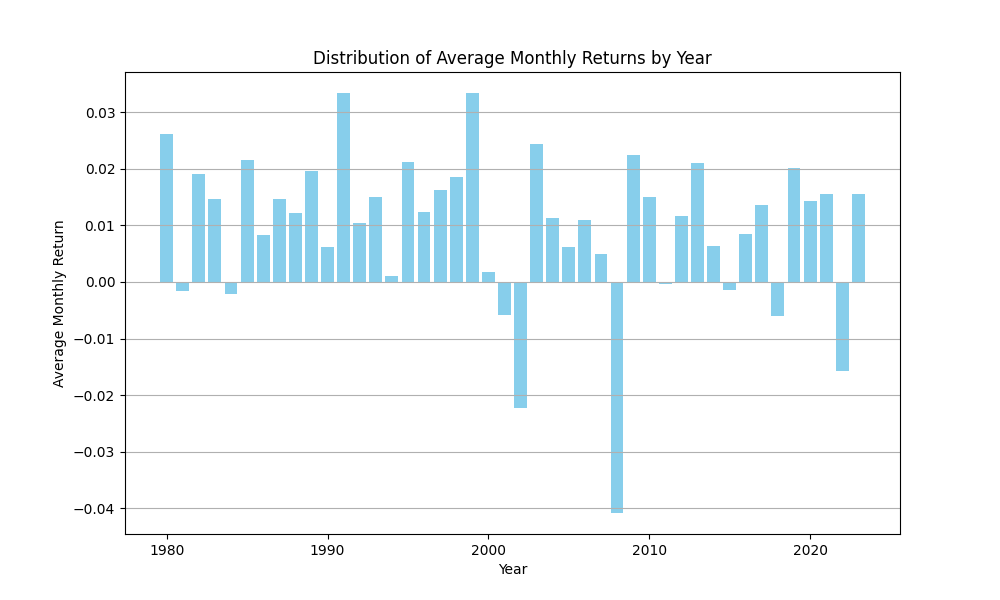
\includegraphics{../data/manual/histogram.png}
    \caption{Yearly average return plot}
    \label{fig:image1}
\end{figure}


\begin{figure}[h]
    \centering
    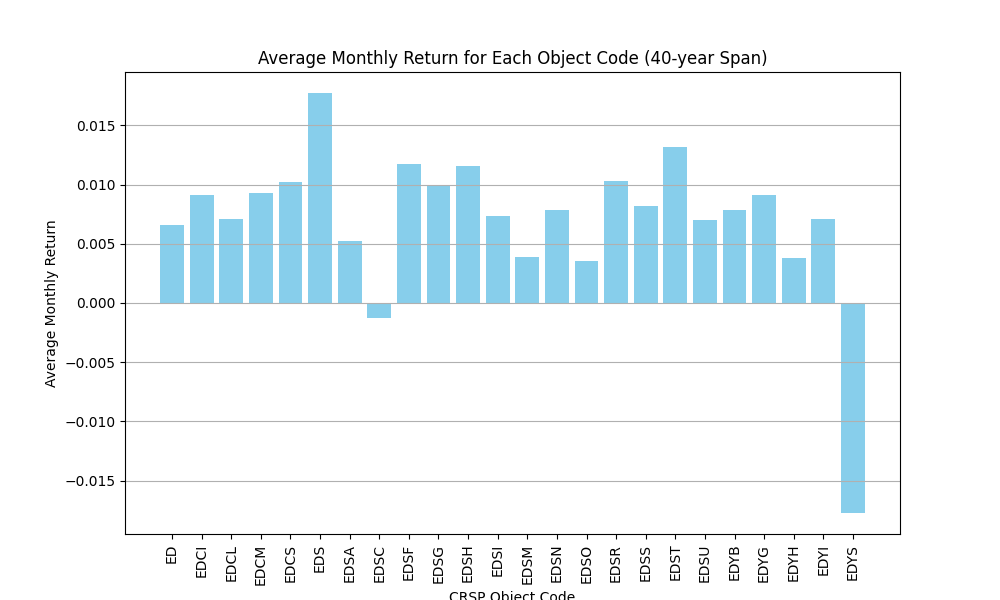
\includegraphics{../data/manual/histogram_mret_per_code.png}
    \caption{Returns by Year and Fund Group Type}
    \label{fig:image2}
\end{figure}

\begin{figure}[h]
    \centering
    
\includegraphics{../data/manual/histogram_code_count.png}
    \caption{Funds Per Object Code}
    \label{fig:image3}
\end{figure}

\begin{table}[ht]
    \centering
    \caption*{Replication of Table 1}
    \label{tab:table_complete}
    \begin{tabular}{lrrrrr}
\toprule
 & year & \multicolumn{2}{r}{$crsp_{TNA}$} & \multicolumn{2}{r}{yret} \\
 &  & mean & median & mean & median \\
\midrule
0 & 1980 & 135.38 & 53.50 & 0.36 & 0.36 \\
1 & 1981 & 154.00 & 55.03 & -0.04 & -0.04 \\
2 & 1982 & 169.27 & 67.98 & 0.24 & 0.25 \\
3 & 1983 & 228.68 & 84.00 & 0.18 & 0.18 \\
4 & 1984 & 225.05 & 79.50 & -0.04 & -0.04 \\
5 & 1985 & 201.82 & 91.90 & 0.27 & 0.27 \\
6 & 1986 & 228.07 & 83.51 & 0.12 & 0.13 \\
7 & 1987 & 222.74 & 66.28 & 0.00 & 0.01 \\
8 & 1988 & 223.77 & 64.01 & 0.14 & 0.14 \\
9 & 1989 & 259.74 & 71.32 & 0.25 & 0.26 \\
10 & 1990 & 362.16 & 106.15 & -0.04 & -0.03 \\
11 & 1991 & 416.54 & 114.86 & 0.34 & 0.31 \\
12 & 1992 & 361.51 & 111.59 & 0.07 & 0.07 \\
13 & 1993 & 429.68 & 113.84 & 0.11 & 0.10 \\
14 & 1994 & 417.67 & 104.85 & -0.01 & -0.01 \\
15 & 1995 & 661.12 & 146.66 & 0.29 & 0.31 \\
16 & 1996 & 882.71 & 170.90 & 0.18 & 0.19 \\
17 & 1997 & 1063.56 & 183.65 & 0.21 & 0.24 \\
18 & 1998 & 1223.19 & 171.00 & 0.13 & 0.13 \\
19 & 1999 & 1390.16 & 179.75 & 0.26 & 0.18 \\
20 & 2000 & 1317.95 & 204.40 & 0.01 & -0.02 \\
21 & 2001 & 1034.07 & 156.35 & -0.10 & -0.11 \\
22 & 2002 & 723.14 & 124.40 & -0.21 & -0.22 \\
23 & 2003 & 1009.79 & 168.10 & 0.34 & 0.31 \\
24 & 2004 & 1137.75 & 200.10 & 0.13 & 0.12 \\
25 & 2005 & 1266.91 & 228.30 & 0.08 & 0.07 \\
26 & 2006 & 1478.86 & 257.70 & 0.15 & 0.13 \\
27 & 2007 & 1248.73 & 210.30 & 0.06 & 0.05 \\
28 & 2008 & 782.02 & 124.90 & -0.38 & -0.38 \\
29 & 2009 & 1120.28 & 190.35 & 0.32 & 0.30 \\
30 & 2010 & 1469.46 & 256.40 & 0.19 & 0.17 \\
31 & 2011 & 1363.40 & 217.70 & -0.03 & -0.02 \\
32 & 2012 & 1567.57 & 243.70 & 0.14 & 0.15 \\
33 & 2013 & 1998.51 & 344.90 & 0.32 & 0.33 \\
34 & 2014 & 2239.81 & 349.05 & 0.08 & 0.08 \\
35 & 2015 & 2097.29 & 290.05 & -0.02 & -0.02 \\
36 & 2016 & 2341.01 & 287.25 & 0.12 & 0.11 \\
37 & 2017 & 2293.50 & 283.70 & 0.18 & 0.18 \\
38 & 2018 & 2189.51 & 247.45 & -0.08 & -0.08 \\
39 & 2019 & 2691.27 & 299.50 & 0.26 & 0.26 \\
40 & 2020 & 2871.09 & 344.10 & 0.17 & 0.14 \\
41 & 2021 & 3439.36 & 399.20 & 0.21 & 0.22 \\
42 & 2022 & 2920.07 & 341.25 & -0.17 & -0.17 \\
43 & 2023 & 3727.34 & 428.20 & 0.19 & 0.17 \\
\bottomrule
\end{tabular}
  
\end{table}
    



\end{document}
